%-----------PREAMBLE-------------------------------------------------------
\documentclass[a4paper]{article}
\usepackage{acro} % used for acronyms
\usepackage{float}
\usepackage{multicol}
\usepackage{titling}
\usepackage{abstract} % sets abstract title on left side
\usepackage{booktabs} % used for table formating
\usepackage{multirow} % table shit
\usepackage{tabulary} % used for table formating
\usepackage[utf8]{inputenc}
\usepackage[english]{babel}
\usepackage{color, colortbl}
\usepackage{graphicx,fancyhdr}
\usepackage[hidelinks]{hyperref}
\usepackage[onehalfspacing]{setspace} % allows double spacing
\usepackage[super,comma,sort&compress]{natbib}
\usepackage[a4paper,margin=2.5cm, headheight=26pt,includeheadfoot]{geometry}
\setlength{\absleftindent}{0pt} %sets abstract title on left side
\setlength{\absrightindent}{0pt} %sets abstract title on left side

%-----------TITLE-------------------------------------------------------
\rhead{McMaster BioMod Team}
\lhead{
\includegraphics[width=1cm]{LogoOnly.png}}
\pagestyle{plain}
\setlength{\droptitle}{-4em}
\title{Controling Chaos: \\ Constructing DNA Nanostructures To Combat Cellular Noise}
%\title{Using DNA Origami As A Protein Scaffold To \\ Enhance Metabolic Production \textit{In Vivo}}
\preauthor{\vspace{-3ex}\begin{center}}
\author{McMaster BioMod Team}
\postauthor{\end{center}}
\predate{}
\date{}
\postdate{}
%\author{McMaster BioMod Team}
%\date{\vspace{-7ex}}

\begin{document}
%\begin{multicols}{2}
\maketitle
\thispagestyle{fancy}
\pagestyle{fancy}

%----------------------------------------------------------
\begin{figure}[H]
    \centering
    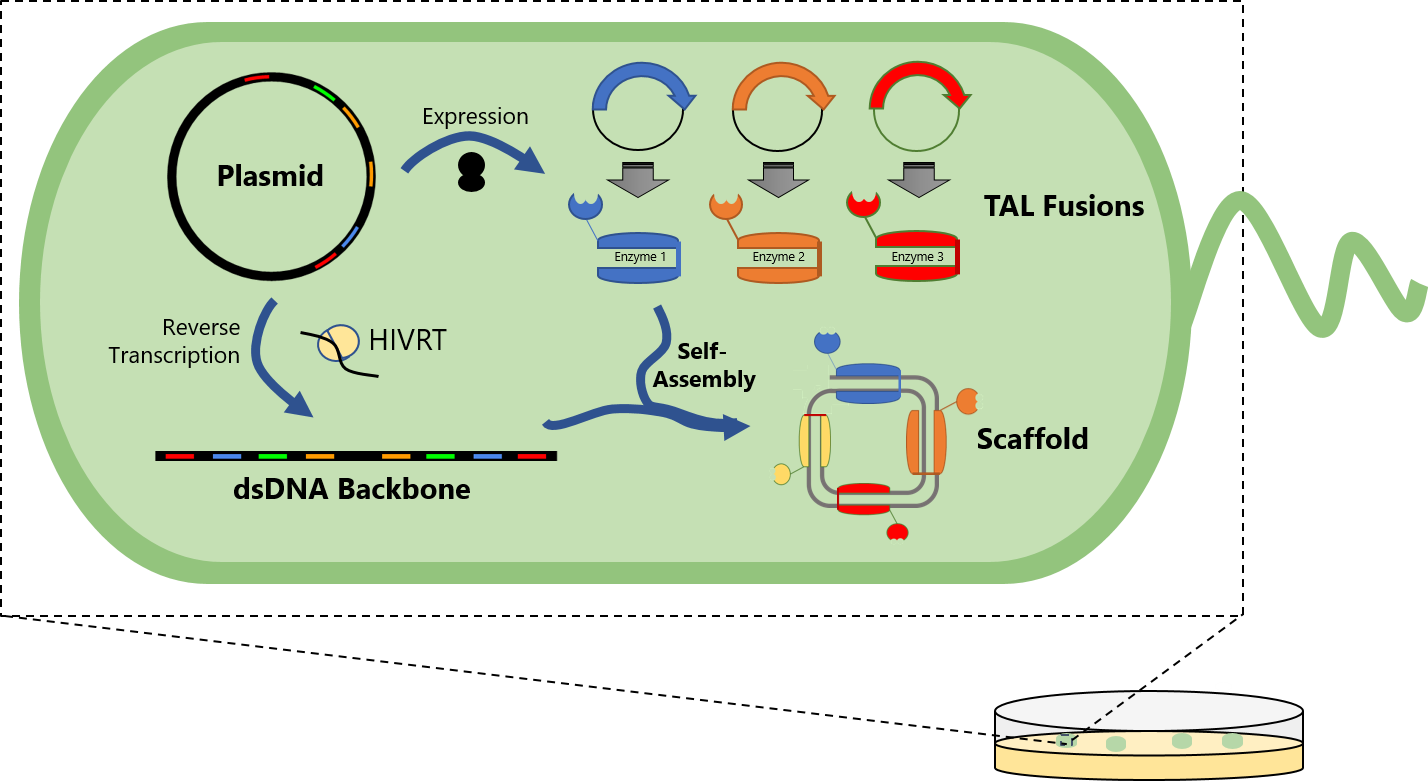
\includegraphics[width=0.9\linewidth]{graphicalAbstract.png}
    \caption{\textbf{Schematic for self-assembly of dsDNA enzymatic scaffolds.} A dsDNA backbone (left) and DNA-binding transcription activator-like (TAL) proteins fused to enzymes (top, right) will be expressed from plasmids using Human Immunodeficiency Virus Reverse-Transcriptase (HIVRT) and regular machinery, respectively. Both components will self-assemble \textit{in vivo} to produce a precise enzymatic scaffold (bottom, right).}
\end{figure}

\begin{abstract}
A major limitation to engineering biological systems are their intrinsic complexity.
Whereas eukaryotes naturally have the advantage of compartmentalized organelles, the prokaryotic models commonly used in synthetic biology often lack such functional organization and thus lack the ability to spatially arrange their cellular components.
To combat this disorganization, we aim to use self-assembling DNA nanostructures to build three-dimensional intracellular scaffolds that enable the control of the spatial organization of functional components – including proteins, RNA, and DNA – by physically placing rate-limiting enzymes in a pathway adjacent to each other\cite{intro1,intro2,intro3,intro4}.
In doing so, the pathway is less limited by the diffusion of reaction intermediates\cite{intro8,intro9}.
To demonstrate this concept, we propose the use of our novel DNA nanostructure scaffolding system to increase the production of the bioplastic P(3HB).
Furthermore, we will build a toolkit to allow both researchers and future iGEM participants to easily integrate DNA nanostructures into any synthetic biology workflow.
Our method has the potential to  drastically increase the efficiency of any existing enzymatic pathways, thus tackling one of the inherent limitations plaguing all synthetic biology projects.
\end{abstract}
\section*{Background \& Rationale}
Many industrially important biosynthesis reactions are limited by the loss of reaction intermediates, suboptimal positioning of involved enzymes, and extra metabolic burden\cite{intro13,intro14}.
Scaffolds, which are naturally used in cells to spatially aggregate complex enzymatic pathways, can be adapted to solve these problems\cite{intro14}.
In the current project, we propose the use of DNA nanostructure scaffolds to control the spatial positioning of catalytic enzymes with nanoscale precision in live cells.
As current ex vivo DNA nanostructure assembly conditions require harsh conditions, we have developed novel methods designed specifically to address this, synthesizing large amounts of double stranded DNA in \textit{E. coli}\cite{intro4}.
When the transcription activator-like (TAL) proteins that recognize a specific sequence are expressed, the TAL proteins will spontaneously fold DNA into DNA/protein nanostructure hybrids\cite{meth2}.
Enzymes could then be kept attached onto individual TAL effectors, thus allowing nanoscale control of protein orientation and position\cite{meth2}.
Our plasmids will be designed in a modular manner, enabling others to easily use our toolkit in projects involving multi-enzyme pathways.
\section*{Objectives}
\begin{itemize}
    \item Produce high yields of dsDNA backbone \textit{in vivo}
    \item Assemble DNA nanostructures \textit{in vitro} and \textit{in vivo}
    \item Assemble a DNA nanostructure scaffold that enhances the efficiency of a three enzyme pathway in bacteria
\end{itemize}
\section*{Methodology}
\subsection*{Producing Large Volumes Of dsDNA}
Synthesizing enough dsDNA for DNA nanostructure assembly \textit{in vivo} has proven to be challenging.
In this project, we propose harnessing the ability of Human Immunodeficiency Virus Reverse-Transcriptase (HIVRT) to produce dsDNA from non-coding RNA (ncRNA) encoded on a plasmid\cite{intro4}.
We will repurpose the method that Elbaz and colleagues have utilized to make ssDNA \textit{in vivo}\cite{meth1}.
A t-RNALys genetic part, which recruits both HIVRT and acts as a transcriptional terminator, will be introduced in front of the sequence encoding the DNA nanostructure strand.
Following the transcription of the RNA encoding the DNA nanostructure subunits, t-RNALys will recruit the two HIVRT subunits and the Monomeric Murine Leukemia Reverse Transcriptase (MLRT) to reverse transcribe the RNA back into dsDNA.
\subsection*{DNA Nanostructure Self-Assembly \textit{in vivo}}
We will first validate the key design features of our project \textit{in vitro} as described by Han and colleagues\cite{meth3}.
In vitro replicability will be established by PCR amplification of both strands of desired DNA nanostructures.
Upon synthesis, the PCR products will be annealed to form their dsDNA sequences, which can then be imaged under Atomic Force Microscopy (AFM) after exposure to a concoction of HIVRT, MLRT and several TAL proteins.
We expect that PCR amplification will produce dsDNA structures of identical morphology.
To test our system \textit{in vivo}, we will transform our plasmid-based expression system into \textit{E.coli}.
Cells will then be lysed and dsDNA will be purified.
Native gel electrophoresis will be employed on extracted dsDNA alongside those generated \textit{in vitro}.
We expect similar pre-folding and post-folding migration patterns for the dsDNA generated \textit{in vitro} and in living cells.
This will be validated by AFM imaging to confirm the expected morphology.
\subsection*{Using DNA Nanostrucures To Enhance The Efficiency of Bioplastic Production}
The ultimate goal of this project is to produce a toolkit that can easily integrate into any synthetic biology project involving an enzymatic pathway.
As a proof of concept, we will improve upon the production of P(3HB), a bioplastic whose synthesis \textit{in vivo} is currently very inefficient in comparison to cell-free methods\cite{plastic}.
The three enzymes used in this biosynthesis pathway, phaA, phaB, phaC, will each be fused to the N-terminal domain of a TAL protein to produce an enzymatic scaffold\cite{plastprod}.
Upon self-assembly of the nanostructure, production of P(3HB) will be measured kinetically to determine the increase in enzymatic efficiency when compared to a non-scaffolded control cell.
\section*{Conclusion}
We propose a novel method for the \textit{in vivo} assembly of dsDNA nanostructures to allow the transferral of  DNA origami applications (such as scaffolding and DNA nanorobots) to the setting of live cells.
To overcome current production bottlenecks of the harsh assembly conditions and the high cost of large-scale DNA synthesis, we utilize (1) a novel reverse transcriptase-based method to generate large amounts of dsDNA \textit{in vivo} and (2) diffusion proteins of TAL effectors and enzymes to create the desired shape while forming an enzyme scaffold.
Therefore, our proposal allows the production of dsDNA origami in a scalable and cost-effective manner.
Notably, we expect this method to give the \textit{in vivo} assembly of dsDNA nanostructures sufficient modularity to be easily used by future researchers and compatible with existing design frameworks.
The proposed technology should thus bridge the gap that limits the application of DNA nanostructures to living biological systems.
%\end{multicols}
\bibliographystyle{naturemag}
\bibliography{refs}
\end{document}

